\section{Discusi\'on}

\subsection{PageRank}
Claramente podemos notar que a medida que el C crece, el algoritmo toma más iteraciones en achicar la norma. Esto se debe a que el grado de aleatoriedad elimina el peso de la unión entre los sitios e indica una uniformidad en el comportamiento, entonces la matriz si bien estocástica ahora se encuentra distribuida esa suma $=$ 1 por columna en varias filas. Esto produce mayor cantidad de iteraciones en el método de la potencia ya que la mayor uniformidad de la matriz provoca que ninguna 'zona' de la matriz absorba más que las demás.   $[1]$
También es bastante notorio que a pesar de que los distintos casos de prueba sean muy diferentes entre si y hasta cientos de veces más grandes, la evolución de la norma converge de formas casi idénticas y lo mismo sucede para las iteraciones requeridas hasta llegar a la norma variando el parámetro c.

La norma Manhattan de la diferencia del vector resultado entre una iteración y la siguiente disminuye tan rápidamente que para visualizarla fue mejor utilizar una escala logarítmica. En las primeras 5 iteraciones la norma disminuye de forma más dramática y a partir de la iteración 10 se puede ver una velocidad de disminución predecible. La diferencia entre una iteración y la otra tiende a disminuirse de forma exponencial.


\subsection{HITS}




\subsection{Ejemplos de comportamiento esperado}

A continuación veremos en redes pequeñas como se comporta el algoritmo para ver si su comportamiento es el esperado.

\subsubsection{HITS}
 \begin{figure}[!htb]
\begin{center}
    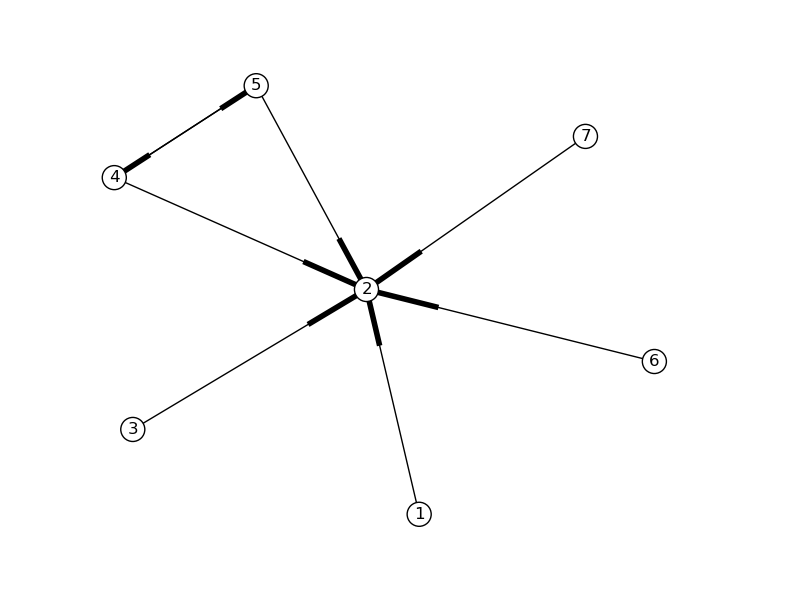
\includegraphics[scale=0.5]{imagenes/test4.png}
    \caption{Red de 7 nodos}
    \end{center}
\end{figure}

Resultado obtenido:
   $$ 
\begin{bmatrix}
              &    Autoridad  &  Hub \\
 Nodo 1 &   0.000000    &      0.383092       \\
 Nodo 2   &  0.967054    &  0.000000     \\
 Nodo 3   &  0.000000   &     0.383092  \\
 Nodo 4   &  0.180008    &     0.454401       \\
 Nodo 5   &  0.180008    &     0.454401        \\
 Nodo 6   &  0.000000    &      0.383092     \\
 Nodo 7   &  0.000000   &     0.383092 \\
\end{bmatrix} 
$$

Efectivamente podemos observar que en la columna de autoridades el nodo 2 es el mayor ya que es el que mas apuntado esta y todos aquellos que tienen 0 es porque no son apuntados por ninguno. Por otro lado en la columna de hubs podemos ver que los nodos 4 y 5 son los que mayor valor tienen ya que son los que mas apuntan a otros nodos con 2 salidas.